
  % ------------------------------------------------------------------------
  % abnTeX2: Modelo de Trabalho Academico (tese de doutorado, dissertacao de
  % mestrado e trabalhos monograficos em geral) em conformidade com
  % ABNT NBR 14724:2011: Informacao e documentacao - Trabalhos academicos -
  % Apresentacao
  % ------------------------------------------------------------------------
  % ------------------------------------------------------------------------

  \documentclass[
    % -- opções da classe memoir --
    12pt,       % tamanho da fonte
    openright,      % capítulos começam em pág ímpar (insere página vazia caso preciso)
    twoside,      % para impressão em verso e anverso. Oposto a oneside
    a4paper,      % tamanho do papel.
    % -- opções da classe abntex2 --
    %chapter=TITLE,   % títulos de capítulos convertidos em letras maiúsculas
    %section=TITLE,   % títulos de seções convertidos em letras maiúsculas
    %subsection=TITLE,  % títulos de subseções convertidos em letras maiúsculas
    %subsubsection=TITLE,% títulos de subsubseções convertidos em letras maiúsculas
    % -- opções do pacote babel --
    english,      % idioma adicional para hifenização
    french,       % idioma adicional para hifenização
    spanish,      % idioma adicional para hifenização
    brazil,       % o último idioma é o principal do documento
    ]{abntex2}


  % ---
  % PACOTES
  % ---

  % ---
  % Pacotes fundamentais
  % ---
  \usepackage{cmap}       % Mapear caracteres especiais no PDF
  \usepackage{lmodern}      % Usa a fonte Latin Modern
  \usepackage[T1]{fontenc}    % Selecao de codigos de fonte.
  \usepackage[utf8]{inputenc}   % Codificacao do documento (conversão automática dos acentos)
  \usepackage{lastpage}     % Usado pela Ficha catalográfica
  \usepackage{indentfirst}    % Indenta o primeiro parágrafo de cada seção.
  \usepackage{color}        % Controle das cores
  \usepackage{graphicx}     % Inclusão de gráficos
  \usepackage{listings}     % Inclusão de código
  \usepackage[final]{pdfpages}
  \usepackage{algorithm}
  \usepackage{algorithmic}
  \usepackage{color}
  \usepackage[section]{placeins}
  \usepackage{csquotes}
  \usepackage{longtable}
  \usepackage[table]{xcolor}
\usepackage{multirow}

  % ---
  % Pacotes de citações
  % ---
  \usepackage[brazilian,hyperpageref]{backref}   % Paginas com as citações na bibl
  \usepackage[alf]{abntex2cite} % Citações padrão ABNT

  % ---
  % CONFIGURAÇÕES DE PACOTES
  % ---

  % ---
  % Configurações do pacote backref
  % Usado sem a opção hyperpageref de backref
  \renewcommand{\backrefpagesname}{Citado na(s) página(s):~}
  % Texto padrão antes do número das páginas
  \renewcommand{\backref}{}
  % Define os textos da citação
  \renewcommand*{\backrefalt}[4]{
    \ifcase #1 %
      Nenhuma citação no texto.%
    \or
      Citado na página #2.%
    \else
      Citado #1 vezes nas páginas #2.%
    \fi}%
    
\renewcommand{\lstlistingname}{Código}
  % ---

  % ---
  % Informações de dados para CAPA e FOLHA DE ROSTO
  % ---
  \titulo{Um estudo de caso de gestão de riscos aplicada a métodos ágeis}
  \autor{Fernanda Narloch Rizzo Hahn}
  \local{Florianópolis}
  \data{2021}
  \orientador{Jean Carlo Rossa Hauck}
  \coorientador{}
  \instituicao{%
    Universidade Federal de Santa Catarina
    \par
    Centro Tecnológico - CTC
    \par
    Departamento de Informática e Estatística
    \par
    Ciências da Computação}
  \tipotrabalho{Dissertação (Bacharelado)}

  \preambulo{Trabalho de Conclusão de Curso submetido ao Curso de
  Ciências da Computação para a obtenção do Grau de Bacharel em
  Ciências da Computação.}
  % ---

  % ---
  % Configurações de aparência do PDF final
    \def\changemargin#1#2{\list{}{\rightmargin#2\leftmargin#1}\item[]}
    \let\endchangemargin=\endlist 

  % alterando o aspecto da cor azul
  \definecolor{blue}{RGB}{41,5,195}

  % informações do PDF
  \makeatletter
  \hypersetup{
        %pagebackref=true,
      pdftitle={\@title},
      pdfauthor={\@author},
        pdfsubject={\imprimirpreambulo},
        pdfcreator={LaTeX with abnTeX2},
      pdfkeywords={abnt}{latex}{abntex}{abntex2}{trabalho acadêmico},
      colorlinks=true,          % false: boxed links; true: colored links
        linkcolor=black,           % color of internal links
        citecolor=black,           % color of links to bibliography
        filecolor=magenta,          % color of file links
      urlcolor=blue,
      bookmarksdepth=4
  }
  \makeatother
  % ---
  % ---
  % Espaçamentos entre linhas e parágrafos
  % ---

  % O tamanho do parágrafo é dado por:
  \setlength{\parindent}{1.3cm}

  % Controle do espaçamento entre um parágrafo e outro:
  \setlength{\parskip}{0.2cm}  % tente também \onelineskip

  % ---
  % compila o indice
  % ---
  \makeindex
  % ---

  % ----
  % Início do documento
  % ----
  \begin{document}
  % Retira espaço extra obsoleto entre as frases.
  \frenchspacing

  % ----------------------------------------------------------
  % ELEMENTOS PRÉ-TEXTUAIS
  % ----------------------------------------------------------
  % \pretextual

  % ---
  % Capa
  % ---
  \imprimircapa
  % ---

  % ---
  % Folha de rosto
  % (o * indica que haverá a ficha bibliográfica)
  % ---
  \imprimirfolhaderosto*
  % ---
  
  % ---
  % Inserir folha de aprovação
  % ---

  % Isto é um exemplo de Folha de aprovação, elemento obrigatório da NBR
  % 14724/2011 (seção 4.2.1.3). Você pode utilizar este modelo até a aprovação
  % do trabalho. Após isso, substitua todo o conteúdo deste arquivo por uma
  % imagem da página assinada pela banca com o comando abaixo:
  %
  % \includepdf{folhadeaprovacao_final.pdf}
  %
  \begin{folhadeaprovacao}

    \begin{center}
      {\ABNTEXchapterfont\large\imprimirautor}

      \vspace*{\fill}
      {\ABNTEXchapterfont\large\bfseries\imprimirtitulo}
      \vspace*{\fill}


     Este Trabalho de Conclusão de Curso foi julgado aprovado para a
     obtenção do Título de Bacharel em Ciências da Computação, e
     aprovado em sua forma final pelo Curso de Ciências da Computação
     da Universidade Federal de Santa Catarina.
     \end{center}

     \assinatura{Dr. Prof. \imprimirorientador \\ Orientador}
     \assinatura{Dr. Prof.  \\ Avaliador}
     \assinatura{Dr. Prof.  \\ Avaliador}
     %\assinatura{\textbf{Professor} \\ Convidado 3}
     %\assinatura{\textbf{Professor} \\ Convidado 4}

     \begin{center}
      \vspace*{0.5cm}
      {\large\imprimirlocal}
      \par
      {\large\imprimirdata}
      \vspace*{1cm}
    \end{center}

  \end{folhadeaprovacao}
  % ---

  % ---
  % Agradecimentos
  % ---
  \begin{agradecimentos}
  \end{agradecimentos}
  % ---

  % ---
  % Epígrafe
  % ---
  \begin{epigrafe}
      \vspace*{\fill}
    \begin{flushright}
      \textit{“As long as you are learning, you are not failing.” – Bob Ross}
    \end{flushright}
  \end{epigrafe}
  % ---

  % ---
  % RESUMOS
  % ---

  % resumo em português
  \begin{resumo}
    A popularização dos métodos ágeis no desenvolvimento de \textit{\textit{software}} trouxe maior velocidade e flexibilidade aos projetos que anteriormente eram desenvolvidos com base em modelos prescritivos. Contudo, os métodos ágeis não são capazes de prevenir por si características típicas de projetos de \textit{software} como a imprevisibilidade e instabilidade. Pois, esses modelos de gerência de projeto não contam com técnicas formais de gestão de riscos para lidar com as incertezas existentes durante o desenvolvimento. Essa lacuna pode provocar o fracasso de um ou mais objetivos do projeto ao preterir a identificação de riscos potencias e consequentemente não dispor de um plano de contingência. Dessa forma, foi criado o “Guia para gestão ágil de riscos em projetos de \textit{software}” no contexto do Grupo de Qualidade de \textit{Software} (GQS/INE/CTC/UFSC) com o intuito de apresentar diretrizes que visam auxiliar a prática da gestão explícita de riscos no ambiente de desenvolvimento ágil de \textit{software}. Assim, o presente trabalho se trata de um estudo de caso que pretende aplicar e avaliar técnicas de gestão de riscos do Guia em equipes ágeis do Laboratório Bridge da Universidade Federal de Santa Catarina. Para isso, inicialmente serão revisados conceitos fundamentais referentes ao tema e também será realizada a análise do estado da arte na área. Com base nos conhecimentos adquiridos e no “Guia para gestão ágil de riscos em projetos de \textit{software}” será desenvolvido um diagnóstico inicial do contexto do Laboratório Bridge e, a partir dele, serão propostas as técnicas a serem aplicadas durante o estudo de caso. Após a implantação das técnicas, será realizada a avaliação dos resultados obtidos.
   \vspace{\onelineskip}

   \noindent
   \textbf{Palavras-chaves}: Gestão de Riscos, Gestão de Projetos, Métodos Ágeis, Desenvolvimento de \textit{Software}
  \end{resumo}

  % resumo em inglês
  \begin{resumo}[Abstract]
   \begin{otherlanguage*}{english}
TODO
     \vspace{\onelineskip}

     \noindent
     \textbf{Key-words}: TODO
   \end{otherlanguage*}
  \end{resumo}
  % ---

  % ---
  % inserir lista de ilustrações
  % ---
  \pdfbookmark[0]{\listfigurename}{lof}
  \listoffigures*
  \cleardoublepage
  % ---

  % ---
  % inserir lista de tabelas
  % ---
  \pdfbookmark[0]{\listtablename}{lot}
  \listoftables*
  \cleardoublepage
  % ---

  % ---
  % inserir lista de abreviaturas e siglas
  % ---
  \begin{siglas}
    \item[PMBOK] Project Management Body of Knowledge
    \item[PMI]  Project Management Institute
    \item[UFSC] Universidade Federal de Santa Catarina
    \item[RSL] Revisão Sistemática da Literatura
 \end{siglas}
  % ---

  % ---
  % inserir o sumario
  % ---
  \pdfbookmark[0]{\contentsname}{toc}
  \tableofcontents*
  \cleardoublepage
  % ---



  % ----------------------------------------------------------
  % ELEMENTOS TEXTUAIS
  % ----------------------------------------------------------
  \textual


  % ----------------------------------------------------------
  % PARTE - preparação da pesquisa
  % ----------------------------------------------------------
\chapter{Introdução e objetivos}
\label{sec:Introducao}
\section{Introdução}

Na busca pela obtenção de vantagens competitivas, surgiu a necessidade de substituir modelos prescritivos por adaptativos no processo de desenvolvimento de \textit{software}. De forma geral, os modelos adaptativos preveem práticas mais flexíveis e com maior enfoque na agilidade, preservando ainda a qualidade do produto \cite{Rech:2013}. Mesmo com essa crescente popularidade das métodos ágeis, o relatório CHAOS Report 2015 conduzido pelo \citeonline{StandishGroup:2014}  apresentou que apenas 39\% dos projetos de \textit{software} que utilizaram métodos ágeis foram bem-sucedidos. Apesar desse cenário e do fato de riscos serem uma constante durante o desenvolvimento de \textit{software} \cite{Cunha:2013}, os método ágeis não contam com uma formalização de técnicas para a gerência de riscos \cite{Tomanek:2015}.

No contexto de gerenciamento de projetos, riscos são uma condição de incerteza que pode ocasionar efeitos positivos ou negativos no projeto \cite{PMBOK:2017}. Segundo o PMBOK, o gerenciamento dos riscos de um projeto tipicamente inclui os processos Planejar o Gerenciamento dos Riscos, Identificar os Riscos, Realizar a Análise Qualitativa dos Riscos, Realizar a Análise Quantitativa dos Riscos, Planejar as Respostas aos Riscos, Implementar Respostas a Riscos e Monitorar Riscos. 

O primeiro se trata do processo para definir qual será a abordagem de gerência de riscos utilizada no projeto. Já Identificar Riscos é o processo de identificar possíveis fontes de risco bem como riscos individuais e documentá-los. Na Análise Qualitativa dos Riscos é realizada a avaliação da probabilidade de ocorrência e impacto de cada risco, a partir disso é possível classificar os riscos quanto a prioridade. A Análise Quantitativa dos Riscos denota o processo de estimar numericamente o efeito combinado dos riscos nos objetivos do projeto. O Planejamento de Respostas aos Riscos é o processo de identificar estratégias de resposta para cada risco identificado, que serão efetuadas no processo Implementar Respostas. Por fim, Monitorar os riscos é o processo de monitorar tanto a implementação das estratégias acordadas, quanto acompanhar os riscos já identificados e identificar novos riscos \cite{PMBOK:2017}.

As técnicas de gerenciamento de riscos possibilitam a redução do impacto negativo e a potencialização do impacto positivo dos riscos \cite{Milare:2019}. Uma pesquisa realizada em 2015, através de entrevistas com gerentes de projeto experientes que utilizam métodos ágeis, concluiu que a gestão proativa de riscos aplicada a modelos adaptativos influencia positivamente o resultado do projeto. E, também pontuou que, apesar dos métodos ágeis já minimizarem os cenários negativos através da aplicação de iterações curtas, a gestão de riscos atua como um complemento, sendo assim, capaz de aperfeiçoar o projeto em questões relacionadas a fatores críticos de sucesso, custo, tempo e qualidade \cite{Gold:2015}.

Diversas iniciativas têm surgido no intuito de auxiliar as organizações de \textit{software} que utilizam métodos ágeis a adotar técnicas explícitas de gestão de riscos. Um desses trabalhos é o “Guia para gestão ágil de riscos em projetos de \textit{software}” desenvolvido no contexto do Grupo de Qualidade de \textit{Software} (GQS/INE/CTC/UFSC). O conteúdo do guia foi fundamentado através da análise da literatura, da identificação do estado da arte na área de gestão ágil de riscos e das experiências empíricas dos autores. E, dispõe de diretrizes que visam auxiliar a prática da gestão explícita de riscos no ambiente de desenvolvimento ágil de \textit{software} \cite{Vieira:2020}. Contudo, o guia ainda não foi aplicado em um contexto real.

A partir do panorama apresentado, este trabalho objetiva realizar um estudo de caso para avaliar o impacto da introdução de práticas explícitas de gerência de riscos no processo de desenvolvimento ágil de \textit{software}. A aplicação do estudo de caso busca selecionar empiricamente quais técnicas utilizadas na gestão de riscos se enquadram melhor no contexto do Laboratório Bridge da Universidade Federal de Santa Catarina, por meio da adoção de técnicas propostas no “Guia para gestão ágil de riscos” \cite{Vieira:2020} em equipes da organização durante o segundo semestre letivo de 2021. O Laboratório Bridge é um laboratório integrado ao Centro Tecnológico (CTC) e de Ciências da Saúde (CCS) da Universidade Federal de Santa Catarina (UFSC) criado em 2013. Atua na pesquisa e desenvolvimento de soluções tecnológicas para o Ministério da Saúde, como por exemplo \textit{softwares} para a estratégia e-SUS APS, Sistema de Monitoramento de Obras (SISMOB) e Registro Nacional de Implantes (RNI). Conta com 123 colaboradores divididos em 6 áreas/projetos, sendo o maior projeto o e-SUS APS com 64 colaboradores distribuídos em 8 equipes ágeis.

Para o desenvolvimento do estudo de caso, primeiramente será realizado um estudo inicial sobre o processo do laboratório bem como a organização desse. Após, utilizando como base a literatura, serão selecionadas técnicas do “Guia para gestão ágil de riscos” \cite{Vieira:2020} que melhor se enquadram com as características do Laboratório Bridge. A cada sprint, uma técnica escolhida será aplicada a uma equipe ágil participante. Ao final da iteração, será avaliado se a técnica trouxe algum benefício para o desempenho da equipe. Dessa forma, será possível definir quais técnicas são mais adequadas ao ambiente ágil do laboratório, bem como quais melhorias essas trouxeram ao processo da organização.

\section{Objetivo geral}

O presente trabalho tem como objetivo geral aplicar e avaliar as técnicas de gestão de riscos presentes no “Guia para gestão ágil de riscos” \cite{Vieira:2020} em um contexto real de desenvolvimento de \textit{software}, por meio de um estudo de caso aplicado a equipes ágeis do Laboratório Bridge da Universidade Federal de Santa Catarina.

\section{Objetivos específicos}
\begin{enumerate}
     \item Realizar uma análise da literatura quanto ao estado da arte da gestão de risco aplicada a métodos ágeis
    \item Realizar um diagnóstico inicial dos processos da unidade organizacional;
    \item Propor técnicas de gestão de risco do “Guia para gestão ágil de riscos” \cite{Vieira:2020} a serem serem aplicadas na unidade organizacional durante estudo de caso;
    \item Avaliar os impactos no processo a partir da aplicação das técnicas e quais técnicas melhor se encaixaram no perfil da unidade organizacional;
\end{enumerate}

\section{Metodologia de pesquisa}

Este trabalho pretende aplicar técnicas de gestão de riscos presentes no “Guia para gestão ágil de riscos”  \cite{Vieira:2020} em uma unidade organizacional e observar, analisar e discutir os impactos dessa aplicação no contexto das equipes ágeis de desenvolvimento de \textit{software}.

Segundo \citeonline{Yin:2001}, “Um estudo de caso é uma investigação empírica que investiga um fenômeno contemporâneo dentro de seu contexto da vida real, especialmente quando os limites entre o fenômeno e o contexto não estão claramente
definidos.”. 

Conforme este conceito de classificação metodológica, o presente trabalho será um estudo de caso, com objetivo exploratório, aplicado dentro de um ambiente real de um laboratório de desenvolvimento de \textit{software}. Para alcançar os objetivos definidos no trabalho, a metodologia adotada foi definida através das três etapas demonstradas a seguir: 

\begin{itemize}[label={}]
  \item \textbf{Etapa 1. Fundamentação Teórica - } Nesta primeira etapa serão revisados conceitos fundamentais da literatura relacionados a gerência de projetos, métodos ágeis e gestão de riscos. As seguintes atividades compõe a etapa:
    \begin{itemize}[label={}]
        \item \textbf{Atividade 1.1 - } Fundamentar principais conceitos sobre gerência de projeto.
        \item \textbf{Atividade 1.2 - } Fundamentar principais conceitos sobre métodos ágeis.
        \item \textbf{Atividade 1.3 - } Fundamentar principais conceitos sobre gestão de riscos. 
    \end{itemize}
  
  
  \item \textbf{Etapa 2. Análise do estado da arte - } A análise do estado da arte possui caráter bibliográfico e objetiva mapear e discutir produções acadêmicas em um campo de conhecimento \cite{Ferreira:2002}. Assim, nesta etapa será realizada uma revisão sistemática da literatura a partir de critérios de pesquisa para o levantamento de estudos correlacionados com o tema deste trabalho. Esta etapa é composta pelas seguintes atividades:
    \begin{itemize}[label={}]
        \item \textbf{Atividade 2.1 - } Especificação do problema.
        \item \textbf{Atividade 2.2 - } Definição das perguntas de pesquisa.
        \item \textbf{Atividade 2.3 - } Identificação dos critérios de pesquisa. 
        \item \textbf{Atividade 2.4 - } Seleção de estudos relacionados a este trabalho. 
        \item \textbf{Atividade 2.5 - } Extração e análise de dados.
    \end{itemize}
  

  \item \textbf{Etapa 3. Definição, aplicação e análise do estudo de caso - } Na terceira e última etapa será planejado e realizado o estudo de caso conforme as atividades abaixo:
      \begin{itemize}[label={}]
        \item \textbf{Atividade 3.1 - } Diagnóstico do contexto da unidade organizacional.
        \item \textbf{Atividade 3.2 - } Definição do estudo.
        \item \textbf{Atividade 3.3 - } Planejamento do estudo. 
        \item \textbf{Atividade 3.4 - } Aplicação do estudo. 
        \item \textbf{Atividade 3.5 - } Análise dos resultados. 
    \end{itemize}

\end{itemize}

\chapter{Fundamentação teórica}
\label{sec:Fundamentacao}

Neste capítulo serão apresentados conceitos relevantes relacionados a gerência de projetos, gestão de riscos e métodos ágeis que serão abordados no decorrer deste trabalho.

\section{Gerência de projetos}

Segundo o PMBOK \cite{PMBOK:2017}: "Projeto é um esforço temporário empreendido para criar um produto, serviço ou resultado único.". Os projetos são de natureza temporária, assim, devem possuir data de início e término definidas. Eles se dão por concluídos quando os objetivos são alcançados ou quando o projeto falha por algum fator como, por exemplo, recursos esgotados, mudança de estratégia ou motivos legais. Um projeto que obtenha sucesso no cumprimento dos objetivos gerará, então, um produto, serviço ou resultado único. 

A área de gerência de projetos objetiva que estes empreendimentos temporários sejam executados de forma eficaz e eficiente. Para que, dessa maneira, as organizações sejam bem sucedidas no cumprimento dos requisitos dos projetos. Este suporte é realizado através da aplicação de conhecimentos, habilidades, ferramentas e técnicas às atividades do projeto \cite{PMBOK:2017}. 

\citeonline{SOMMERVILLE:2011} considera a gerência de projetos uma peça fundamental da engenharia de \textit{software}. Para ele, apesar do bom gerenciamento do projeto não resultar necessariamente no sucesso do projeto, o mau gerenciamento costuma ocasionar a falha do empreendimento. 

Assim, para garantir um bom gerenciamento de projeto e assim aumentar as chances de sucesso, o PMBOK \cite{PMBOK:2017} identifica componentes-chave que devem ser gerenciados. Tais componentes estão descritos na Tabela \ref{tab:KeyComponents}.

\begin{longtable}{|p{5cm}|p{10cm}|}
    \caption{Descrição dos componentes-chave do Guia PMBOK}
    \label{tab:KeyComponents}
              \centering
              \cr \rowcolor{lightgray}
              \textbf{Componentes-Chave} & \textbf{Descrição} 
              \\ \hline 
              \textbf{Ciclo de vida do projeto} &
              A série de fases pelas quais um projeto passa, do início ao término.
              \\ \hline
              
              \textbf{Fase do projeto} &
              Um conjunto de atividades do projeto relacionadas de maneira lógica que culmina na conclusão de uma ou mais entregas
              \\ \hline 
              
                
              \textbf{Revisão de fase} &
              Uma análise no final de uma fase em que uma decisão é tomada em relação a passar para a fase seguinte, continuar com modificações ou finalizar um programa ou projeto.
              \\\hline 
              
              \textbf{Processos de gerenciamento de projetos} &
              Uma série de atividades sistemáticas direcionadas para alcançar um resultado final de tal forma que se aja em relação a uma ou mais entradas a fim de criar uma ou mais saídas.
              \\\hline 
              
              \textbf{Grupo de processos de gerenciamento de projetos} &
              Um agrupamento lógico de entradas, ferramentas, técnicas e saídas de gerenciamento de projetos. Os grupos de processos de gerenciamento de projetos incluem iniciar, planejar, executar, monitorar, controlar e encerrar. Os grupos de processos de gerenciamento de projetos não são fases do projeto.
              \\\hline 
              
              \textbf{Área de conhecimento em gerenciamento de projetos} &
              Uma área identificada de gerenciamento de projetos definida por seus requisitos de conhecimentos e descrita em termos dos processos que a compõem: suas práticas, entradas, saídas, ferramentas e técnicas.
              \\\hline 
                 
              \caption*{\textbf{Fonte:} Adaptado de PMBOK \cite{PMBOK:2017}}
\end{longtable}

Esses conceitos-chave são inter-relacionados, assim, o ciclo de vida contém as fases pelos quais o projeto passa. Ele fornece, portanto, a estrutura básica para o gerenciamento do projeto. As fases são um conjunto de atividades descritas por atributos tais quais nome da fase, número de fases, duração, requisitos de recursos e critérios de entrada e saída. O processo de revisão de fase ocorre ao fim de uma fase e resulta em uma decisão que pode ser prosseguir para a fase seguinte, terminar o projeto, continuar na fase ou repeti-la.

Para a gerência do ciclo de vida do projeto, são utilizados processos de gerenciamento de projeto. Eles são atividades que produzem uma ou mais saídas de uma ou mais entradas. As saídas podem ser tanto uma entrada para outro processo quanto uma entrega ou fase do projeto. Alguns exemplos de processos são: Desenvolver o Termo de Abertura do Projeto, Adquirir Recursos e Definir as Atividades. E, esses podem ser divididos em processos utilizados apenas uma vez, processos periódicos ou conforme a necessidade e processos contínuos \cite{PMBOK:2017}.

Além disso, o PMBOK \cite{PMBOK:2017} apresenta cinco Grupos de Processo de Gerenciamento de Projetos e dez Áreas de Conhecimento em Gerenciamento de Projetos, que categorizam os processos de gerenciamento. Os grupos de processo são organizados da seguinte forma:

\begin{itemize}
    \item \textbf{Grupo de processos de iniciação:} São os processos dedicados a obter a aprovação para novos projetos ou fases de projeto. Esses processos são responsáveis por auxiliar as partes interessadas a avaliar a viabilidade do projeto e alinhar as expectativas quanto aos resultados.
    \item \textbf{Grupo de processos de planejamento:} Esse grupo é composto por processos para refinar os objetivos traçados na iniciação e definir um escopo de trabalho para o projeto.
    \item \textbf{Grupo de processos de execução:} Envolve os processos necessários para concluir os trabalhos definidos no planejamento. 
    \item \textbf{Grupo de processos de monitoramento e controle:} Está relacionando com o acompanhamento da evolução do projeto, através da análise do desempenho e a identificação de possíveis modificações.
    \item \textbf{Grupo de processos de encerramento:} Processos que formalizam o encerramento do projeto, fase ou contrato.
\end{itemize}

Já as áreas de conhecimento identificadas pelo PMBOK \cite{PMBOK:2017} categorizam os processos em requisitos de conhecimento. As áreas de conhecimento são dispostas da seguinte forma:

\begin{itemize}
    \item \textbf{Gerenciamento da integração do projeto:} São processos que unificam e coordenam as atividades dos Grupos de Processos de Gerenciamento do Projeto. Esses processos são aplicados durante todo o ciclo de vida do projeto.
    \item \textbf{Gerenciamento do escopo do projeto:} Os processos do gerenciamento de escopo definem aquilo que está ou não incluído no projeto. Eles garantem que o projeto envolva todo o trabalho necessário para que os objetivos sejam atingidos.
    \item \textbf{Gerenciamento do cronograma do projeto:} Inclui os processos necessários para assegurar que o projeto cumprirá os prazos definidos.
    \item \textbf{Gerenciamento dos custos do projeto:} Esses processos têm como objetivo garantir que o projeto seja finalizado dentro do orçamento.
    \item \textbf{Gerenciamento da qualidade do projeto:} Garantem que tanto o processo de gerenciamento de projeto quanto o produto atendem à critérios de qualidade condizentes com as expectativas das partes interessadas.
    \item \textbf{Gerenciamento dos recursos do projeto:} Engloba os processos responsáveis por enumerar, adquirir e gerenciar os recursos essenciais para o sucesso do projeto.
    \item \textbf{Gerenciamento das comunicações do projeto:} São processos que endossam a coleta, armazenamento e distribuição de informações importantes para o projeto.
    \item \textbf{Gerenciamento dos riscos do projeto:} Inclui os processos responsáveis por minimizar ameaças ao desenvolvimento do projeto bem como maximizar as oportunidades.
    \item \textbf{Gerenciamento das aquisições do projeto:} É a área responsável por obter produtos ou serviços externos à equipe do projeto.
    \item \textbf{Gerenciamento das partes interessadas do projeto:} Inclui os processos que identificam as partes interessadas no projeto e também planejam, gerenciam e monitoram o envolvimento de cada uma delas com o projeto.
\end{itemize}

A Figura \ref{interrelacaoConceitos} demonstra as inter-relações dos conceitos-chave apresentados anteriormente:

\begin{figure}[h]
    \centering
    \caption{Inter-relação dos componentes-chave do Guia PMBOK}
    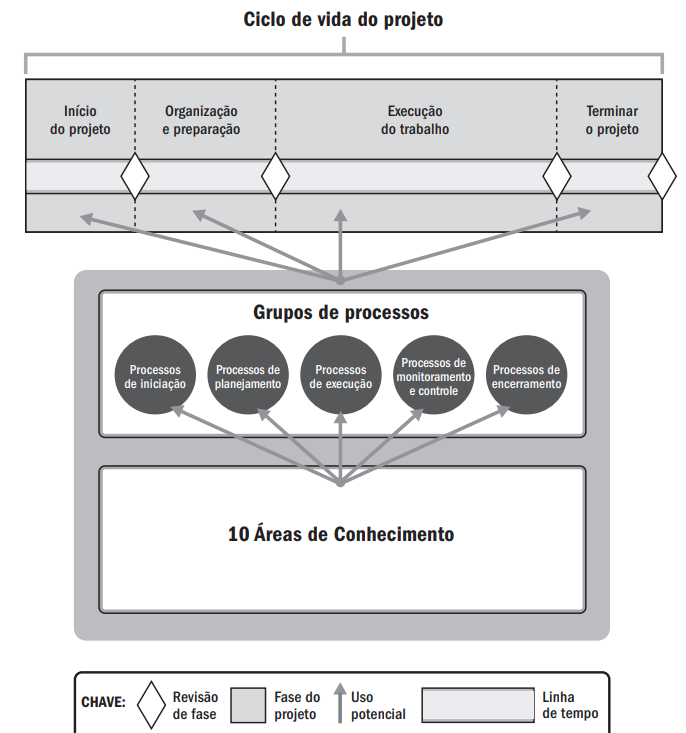
\includegraphics[scale=0.47]{src/tex/img/interrelacaoPMBOKpg18.png} \\
    \label{interrelacaoConceitos}
    \textbf{Fonte:} PMBOK \cite{PMBOK:2017}
    \centering
\end{figure}

É importante salientar que o gerenciamento de projetos na área de desenvolvimento de \textit{software} possui certas particularidades que podem trazer desafios. Como por exemplo, o fato de que os produtos desenvolvidos são intangíveis, ou seja não são tão explícitos como, por exemplo, um projeto de engenharia civil. Assim, partes inacabadas do projeto podem mais facilmente passarem despercebidas. Além disso, projetos de \textit{software} são muito distintos entre si, então até mesmo gerentes com grande experiência podem ter dificuldades em prever problemas. Mais, os processos de desenvolvimento de \textit{software} variam de organização para organização \cite{SOMMERVILLE:2011}.

O SWEBOK \cite{SWEBOK:2014} também enfatiza que existe um distanciamento entre os clientes e os processos necessários para desenvolver \textit{software}, tornando difícil que esses compreendam a complexidade do projeto. As contantes mudanças de requisitos são outra particularidade da área, que exige que o \textit{software} seja construído através de processos iterativos. Outras diferenças importantes são sobre a necessidade de se balancear criatividade e disciplina dentro do processo bem como o grau de complexidade de desenvolvimento e a exigência de constante atualização técnica das equipes.

\section{Gestão de riscos}

Em 1983, a Royal Society britânica publicou um relatório denominado \textit{"Risk assessment: a Study Group Report"}, que definiu risco como: A probabilidade de que um determinado evento adverso ocorra durante um período de tempo definido ou resulte de determinado desafio. Como na probabilidade no sentido da teoria estatística, o risco obedece a todas as leis formais das probabilidades combinatórias \cite{ADAMS:1995}. 

Já o PMBOK \cite{PMBOK:2017} inclui neste conceito a possibilidade de que riscos tenham também um efeito positivo no projeto. No guia são definidos dois tipos de risco: o risco individual do projeto e o risco geral do projeto. Para o PMBOK, o primeiro "é um evento ou condição incerta que, se ocorrer, provocará um efeito positivo ou
negativo em um ou mais objetivos do projeto.". E o risco geral do projeto " é o efeito da incerteza do projeto no seu todo, decorrente de todas as fontes de incerteza, incluindo riscos individuais, representando a exposição das partes interessadas às implicações de variações no resultado do projeto, sejam positivas ou negativas."

\citeonline{SOMMERVILLE:2011} ainda cita três categorias de risco relacionados a projetos de \textit{software}, são elas:

\begin{itemize}
    \item\textbf{Riscos de projeto:} São incertezas que podem impactar o cronograma ou os recursos do projeto.  
    \item\textbf{Riscos de produto:} Os riscos relacionados ao \textit{software} sendo desenvolvido, capazes de afetar a qualidade do produto.
    \item\textbf{Riscos de negócio:} Riscos que afetam a organização.
\end{itemize}

Essas categorias de riscos se sobrepõe, ou seja, um risco pode pertencer a uma ou mais categoria concomitantemente. \citeonline{SOMMERVILLE:2011} cita como exemplo a saída de um desenvolvedor experiente do time. Esse risco pode se enquadrar em risco de projeto, produto e também negócio. 

O motivo para isso é que quando o time perde um membro experiente é quase certo de que haverá uma queda na produtividade. Mesmo que o desenvolvedor seja substituído, o novo membro do projeto ainda levará tempo para aprender a realizar as tarefas. Então, tal risco possivelmente gerará um atraso no cronograma. Mais ainda, a saída de um colaborador experiente pode deixar uma lacuna de conhecimento no time e, assim, aumentam as chances de serem cometidos erros de programação. A perda da qualidade do \textit{software} enquadraria o risco em risco de produto. Por fim, a saída do programador pode ser um risco de negócio ao passo que a experiência do desenvolvedor pode ser crucial para o fechamento de novos contratos.

Para \citeonline{WAZLAWICK:2013}, os riscos estão presentes em todos os projetos de desenvolvimento de \textit{software} e, caso não se esteja atento a eles, os riscos podem prejudicar ou até mesmo inviabilizar um projeto. Ademais, de uma maneira genérica, é possível afirmar que negligenciar o planejamento em relação aos riscos é uma das maiores razões para o insucesso de um projeto de \textit{software}.

A partir desse contexto, a motivação para a gestão de risco se dá pelo fato de que riscos negativos (ameaças) não administrados podem gerar efeitos negativos no projeto, ou então, podem ser perdidos riscos positivos (oportunidades) não identificados. Portanto, o objetivo da gestão de risco é potencializar as oportunidades e minimizar as ameaças \cite{PMBOK:2017}.

Para obter tais benefícios a partir da gestão de riscos, \citeonline{HOPKIN:2010} destaca a importância de não apenas identificar e avaliar os riscos, mas também utilizar essas informações para tomar decisões mais embasadas e criar planos apropriados de resposta aos riscos. 

Esse processo completo foi formalizado pelo PMBOK \cite{PMBOK:2017} através da definição de sete processos de gerenciamento de riscos. São eles: Planejar o Gerenciamento de Riscos, Indentificar os Riscos, Realizar a Análise Qualitativa dos Riscos, Realizar a Análise Quantitativa dos Riscos, Planejar Respostas aos Riscos, Implementar Respostas a Riscos e Monitorar os Riscos. Cada um deles é apresentado com mais detalhes nas subseções a seguir.

\subsection{Planejar o Gerenciamento dos Riscos}

Segundo o \cite{PMBOK:2017}, o primeiro passo no processo de gerenciamento de risco é definir como serão conduzidas as atividades de gerenciamento. A definição é feita na concepção do projeto e deve estar concluída no início do projeto. Contudo, o processo pode ser revisitado caso ocorra, por exemplo, uma grande mudança no escopo do projeto.

Para a realização do Planejamento do Gerenciamento dos Riscos, o \citeonline{PMBOK:2017} prevê as seguintes entradas:

\begin{itemize}
    \item\textbf{Termo de abertura do projeto:} O documento que formaliza o início do projeto e descreve sem riqueza de detalhes os limites, requisitos e riscos do projeto.  
    \item\textbf{Plano de gerenciamento do projeto:} Para que o plano de gerenciamento de riscos seja coerente, deve-se levar em consideração os todos os planos de gerenciamento do projeto aprovados.
    \item\textbf{Documento do projeto:} O documento de projeto utilizado de entrada para essa fase pode ser o registro das partes interessadas, pois a partir desse documento é possível formalizar o papel de cada uma das partes dentro do projeto. E, assim, definir os responsáveis pelo gerenciamento de risco.
    \item\textbf{Fatores ambientais da empresa:} Fatores que podem impactar o planejamento como os limites gerais de riscos definidos pela organização.
    \item\textbf{Ativos de processos organizacionais:} Ativos que podem influenciar o processo de planejar o gerenciamento, como papéis e responsabilidades e a política organizacional de riscos.
\end{itemize}

Já as ferramentas e técnicas a serem utilizadas delimitadas pelo \citeonline{PMBOK:2017} são a \textbf{opinião especializada}, a \textbf{análise de dados} e \textbf{reuniões}. A primeira se refere ao aproveitamento da expertise de pessoas ou grupos em assuntos relacionados a gerenciamento de risco. A análise de dados trata em especial da análise das partes interessadas. E, por fim, as reuniões de início de projeto ou reuniões de planejamento podem incluir o desenvolvimento do \textbf{plano de gerenciamento de risco}.

O \textbf{plano de gerenciamento de risco} é a saída esperada dessa fase e pode incluir elementos como:

\begin{itemize}
    \item Estratégia dos riscos
    \item Metodologia
    \item Papéis e responsabilidades
    \item Financiamento
    \item Prazos
    \item Categoria dos riscos
    \item Apetite a riscos das partes interessadas
    \item Definições de probabilidade e impacto dos riscos
    \item Matriz de probabilidade e impacto
    \item Formatos de relatórios
    \item Acompanhamento
\end{itemize}

\subsection{Identificar os Riscos}

Sobre a identificação de riscos, \citeonline{PRESSMAN:2011} afirma que:

\begin{changemargin}{4cm}{0cm}
\begin{footnotesize}
A identificação do risco é uma tentativa sistemática para especificar ameaças ao plano do projeto (estimativas, cronograma, recursos etc.). Identificando os riscos conhecidos e previsíveis, o gerente de projeto dá o primeiro passo no sentido de evitá-los quando possível e controlá-los quando necessário.
\end{footnotesize}
\end{changemargin}

Assim, o objetivo desse processo é identificar os riscos individuais e fontes de risco. A partir da identificação, documenta-se as características dos riscos encontrados. Dessa forma, é possível agregar informações importantes para que a equipe do projeto possa responder adequadamente aos riscos \cite{PMBOK:2017}.

É importante destacar que a identificação de riscos é um processo iterativo e deve ocorrer ao longo do projeto. Além disso, todas as partes interessadas do projeto devem ser incentivadas a participar da identificação dos riscos \cite{PMBOK:2017}. 

Segundo \citeonline{WAZLAWICK:2013}, também é recomendável que os responsáveis pela identificação de riscos tenham acesso a um catálogo de riscos identificados em projetos semelhantes anteriores. 

Existem diversas maneiras de identificar os riscos individuais do projeto, entre elas estão o uso de \textit{checklists} predefinidos que podem ser obtidos na literatura ou na \textit{Internet}, reuniões e \textit{brainstormings} e a análise de cenários de projetos semelhantes anteriores \cite{WAZLAWICK:2013}.

O \citeonline{PMBOK:2017} também cita algumas entradas que podem ser utilizadas de apoio para a identificação de riscos, como o plano de gerenciamento de risco, documentos do projeto, acordos, documentação de aquisições, fatores ambientais da empresa e ativos de processos organizacionais.

As saídas esperadas desse processo são o registro dos riscos identificados, que deve seguir um formato uniforme para garantir a clareza e compreensão dos riscos, e o relatório de riscos \cite{PMBOK:2017}. 

\subsection{Realizar a Análise Qualitativa dos Riscos}

Os riscos agora identificados precisam passar por uma análise para se determinar a importância de cada um deles, com o objetivo de determinar quais são os realmente relevantes para que sejam aplicados recursos na prevenção \cite{WAZLAWICK:2013}.

A análise \textbf{qualitativa} dos riscos é subjetiva, ou seja, baseia-se na percepção dos membros da equipe do projeto. Através dessa análise são priorizados os riscos, utilizando como parâmetro a probabilidade e o impacto da ocorrência \cite{PMBOK:2017}.

Esse processo, assim como a identificação de riscos, é iterativo e é realizado à medida que novos riscos são identificados. O objetivo desse processo é garantir que seja demandado maior esforço nos riscos considerados mais prioritários \cite{PMBOK:2017}.

Algumas ferramentas e técnicas sugeridas pelo \citeonline{PMBOK:2017} são opinião especializada, técnicas de coleta de dados como entrevistas, análise de dados, o uso de um facilitador, categorização dos riscos e reuniões.

\subsection{Realizar a Análise Quantitativa dos Riscos}



\subsection{Planejar Respostas aos Riscos}
\subsection{Implementar Respostas aos Riscos}
\subsection{Monitorar Riscos}

\section{Métodos ágeis}

Na década de 1980 e início de 1990, acreditava-se que o processo de desenvolvimento de \textit{software} deveria ser minuciosamente planejado e monitorado. Tal noção advém principalmente dos primórdios da engenharia de \textit{software}, que surgiu dentro de um contexto de \textit{softwares} robustos e duradouros como sistemas aeroespaciais e \textit{softwares} de governo. \cite{SOMMERVILLE:2011}.

Porém, esse métodos chamados de prescritivos, quando aplicados a \textit{softwares} corporativos de portes pequenos e médios, acabam prejudicando o andamento do projeto. Isso ocorre porque gasta-se mais tempo no planejamento e análise do projeto do que de fato no desenvolvimento. Além disso, tais sistemas frequentemente possuem requisitos mutáveis, o que envolve modificações no código e a adaptação das especificações. \cite{SOMMERVILLE:2011}.

\citeonline{COCKBURN:2002} argumenta que os métodos prescritivos falham ao assumir que as engenheiros de \textit{software} são máquinas. Ou seja, eles não consideram as fragilidades dos seres humanos, tais quais: diferentes estilos de trabalho, níveis de habilidades, concentração e criatividade. Além disso, erram ao assumir total disciplina e consistência por partes dos colaboradores durante um período longo de projeto.

Neste cenário de insatisfação, surgiram os métodos ágeis que possuem como principal característica a utilização de uma abordagem incremental tanto para a especificação do sistema quanto para o desenvolvimento e entrega. Assim, os métodos ágeis permitem que os \textit{softwares} sejam rapidamente entregues e facilmente adaptáveis a novos requisitos \cite{SOMMERVILLE:2011}.

A filosofia dos métodos ágeis foi descrita em 2001 por um grupo de 17 desevolvedores de \textit{software} através do Manifesto Ágil \cite{AGILEMANIFEST:2001}. Tal manifesto possui quatro valores:

\begin{itemize}
        \item Indivíduos e interações mais que processos e ferramentas;
        \item \textit{Software} em funcionamento mais que documentação abrangente;
        \item Colaboração com o cliente mais que negociação de contratos;
        \item Responder a mudanças mais que seguir um plano;
\end{itemize}

E, embora processos e ferramentas, documentação abrangente, negociação de contratos e seguir um plano sejam importantes, o manifesto valoriza mais os pontos à esquerda: Indivíduos e interações, \textit{software} em funcionamento, colaboração com o cliente e resposta à mudanças. No livro Engenharia de \textit{Software}, \citeonline{WAZLAWICK:2013} salienta que a cultura ágil não abandona planejamento, modelagem, documentação e ferramentas, ela apenas valoriza os pontos mais essenciais de um projeto de \textit{software}.

\citeonline{PRESSMAN:2011} também reforça esse ponto ao destacar que os métodos ágeis não são a antítese da engenharia de \textit{software} e sim um complemento a ser aplicado nos projetos. Ou seja, os métodos ágeis funcionam como uma filosofia para os trabalhos de \textit{software}.

Além dos quatro valores, o Manifesto Ágil \cite{AGILEMANIFEST:2001} também é composto por doze princípios: 

\begin{itemize}
        \item Nossa maior prioridade é satisfazer o cliente através da entrega contínua e adiantada de \textit{software} com valor agregado.
        \item Mudanças nos requisitos são bem-vindas, mesmo tardiamente no desenvolvimento. Processos ágeis tiram vantagem das mudanças visando vantagem competitiva para o cliente.
        \item Entregar frequentemente \textit{software} funcionando, de poucas semanas a poucos meses, com preferência à menor escala de tempo.
        \item Pessoas de negócio e desenvolvedores devem trabalhar diariamente em conjunto por todo o projeto.
        \item Construa projetos em torno de indivíduos motivados. Dê a eles o ambiente e o suporte necessário e confie neles para fazer o trabalho.
        \item O método mais eficiente e eficaz de transmitir informações para e entre uma equipe de desenvolvimento é através de conversa face a face.
        \item \textit{Software} funcionando é a medida primária de progresso.
        \item Os processos ágeis promovem desenvolvimento sustentável. Os patrocinadores, desenvolvedores e usuários devem ser capazes de manter um ritmo constante indefinidamente.
        \item Contínua atenção à excelência técnica e bom design aumenta a agilidade.
        \item Simplicidade - a arte de maximizar a quantidade de trabalho não realizado - é essencial.
        \item As melhores arquiteturas, requisitos e designs emergem de equipes auto-organizáveis.
        \item Em intervalos regulares, a equipe reflete sobre como se tornar mais eficaz e então refina e ajusta seu comportamento de acordo.
\end{itemize}

Ao refletir sobre o Manifesto Ágil \cite{AGILEMANIFEST:2001}, \citeonline{PRESSMAN:2011} define agilidade como algo que envolve, além de rápidas respostas à mudança, a entrega rápida de \textit{softwares} em funcionamento, a participação do cliente nas fases do projeto, maior facilidade de comunicação e estruturação na equipe e reconhecimento da necessidade de ser flexível quanto aos planos.

Métodos ágeis são um termo geral para uma gama de \textit{frameworks} e técnicas \cite{PMIAGILE:2017}. Portanto, cada método ágil utiliza processos distintos para instanciar os princípios da filosofia ágil demonstrados no Manifesto Ágil \cite{AGILEMANIFEST:2001}. Mesmo assim, os métodos ágeis possuem alguns pontos importantes em comum, explicitados na tabela abaixo:

\begin{longtable}{|p{5cm}|p{10cm}|}
    \caption{Princípios compartilhados pelos métodos ágeis}
    \label{tab:KeyComponents}
    \centering
            \centering
            \cr \rowcolor{lightgray}
            \textbf{Princípios} & \textbf{Descrição}
            \\ \hline
              
            \textbf{Envolvimento do cliente} &
            Os clientes devem estar intimamente envolvidos no processo de desenvolvimento. Seu papel é fornecer e priorizar novos requisitos do sistema e avaliar suas iterações.
            \\\hline
              
            \textbf{Entrega incremental} &
            0 software é desenvolvido em incrementos com o cliente, especificando os requisitos para serem incluídos em cada um.
            \\\hline
              
            \textbf{Pessoas, não processos} &
            As habilidades da equipe de desenvolvimento devem ser reconhecidas e exploradas. Membros da equipe devem desenvolver suas próprias maneiras de trabalhar, sem processos prescritivos.
            \\\hline 
              
            \textbf{Aceitar as mudanças} &
            Deve-se ter em mente que os requisitos do sistema vão mudar. Por isso, projete o sistema de maneira a acomodar essas mudanças.
            \\\hline 
              
            \textbf{Manter a simplicidade} &
            Focalize a simplicidade, tanto do software a ser desenvolvido quanto do processo de desenvolvimento. Sempre que possível, trabalhe ativamente para eliminar a complexidade do sistema.
            \\\hline
              
            \caption*{\textbf{Fonte:} Adaptado de \citeonline{SOMMERVILLE:2011}}
\end{longtable}

A Figura \ref{metodosAgeis} destaca algumas abordagens ágeis conhecidas e o compartilhamento de princípios e valores entre elas.

\begin{figure}[h]
    \centering
    \caption{Métodos ágeis}
    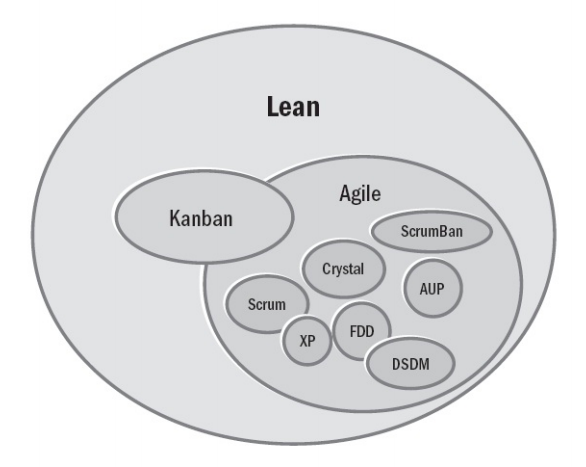
\includegraphics[scale=0.5]{src/tex/img/metodosageisPMI.png}\\
    \label{metodosAgeis}
    \textbf{Fonte:} \textit{Agile Practice Guide} \cite{PMIAGILE:2017}
\end{figure}

Nas subseções seguintes alguns dos métodos ágeis serão apresentados e elucidados.

\subsection{ \textit{Lean} }

A abordagem \textit{Lean} proposta inicialmente pela Toyota é em primeiro lugar um sistema humano e não apenas focado em cerimônias e artefatos. Ou seja, ela coloca em foco os colaborados da empresa e dá mais autonomia a eles. Essa filosofia de produção é importante para o cenário tecnológico atual ao considerar as constantes mudanças e incertezas, através da maximização do potencial humano \cite{LEANENT:2016}.

Apesar do \textit{Lean} ter sido fundamentado na indústria automobilística ele foi adaptado à indústria de software. E, nestes dias, é denominado \textit{Lean Software Development}, termo foi utilizado pela primeira vez por Tom e Mary Poppendieck \cite{WAZLAWICK:2013}.

\citeonline{Poppendieck:2006} também desenharam os princípios do \textit{Lean} para desenvolvimento de \textit{software}. São eles:

\begin{itemize}
    \item \textbf{Eliminar o desperdício:} No desenvolvimento de \textit{software} podem ser identificados diversos desperdícios, por exemplo: funcionalidades extras, levantar requisitos ou realizar testes muito cedo. Para isso, é necessário despender esforços apenas com o necessário e com o que agregue valor ao cliente.
    \item \textbf{Criar conhecimento:} Realizar ciclos de \textit{feedback}, utilizar o método científico e estimular a busca por conhecimento dentro da organização. 
    \item \textbf{Decidir tardiamente:} Ter em mente que os requisitos podem mudar e não é necessário aguardar a especificação completa para iniciar o desenvolvimento.     
    \item \textbf{Entregar o mais rápido possível:} Desenvolver \textit{software} em ciclos curtos e incrementais. E, dessa forma, garantir entregas frequentes e evitar atrasos.
    \item \textbf{Respeitar as pessoas:} Engajar e empoderar o time através de respeito mútuo e confiança.
    \item \textbf{Otimizar o todo:} Considerar o todo e não apenas as partes do \textit{software} que estão sendo desenvolvidas no momento.
    \item \textbf{Manter a qualidade:} Priorizar um código modular e incremental, evitar permanecer desenvolvendo código legado e focar nos cenários de teste.
\end{itemize}

Assim, a filosofia \textit{Lean} agrega a base para outros métodos ágeis como XP, Scrum, Kanban e Scrumban ao instaciar conceitos como foco no valor, entregas pequenas e eliminação de desperdício \cite{PMIAGILE:2017}.

\subsection{XP}

\textit{Extreme Programming} (XP) é um método utilizado desde o final da década de 80, quando teve os conceitos iniciais definidos. Porém, esse método ágil foi formalizado apenas nos anos 2000 por Kent Beck. Inicialmente, o XP era apenas aplicado em pequenas e médias equipes, porém alguns anos depois foi proposta a variação do XP, chamada \textit{Industrial XP} (IXP). Essa, por sua vez, permite a aplicação de um processo ágil em organizações de grande porte \cite{PRESSMAN:2011}. 

\citeonline{WAZLAWICK:2013} enumera os principais valores de XP da seguinte forma:

\begin{itemize}
    \item \textbf{Simplicidade:} Deve-se focar apenas nos requisitos necessários para o projeto. Ou seja, mirar em um produto simples que oferece aquilo que sabe-se que o cliente necessita.
    \item \textbf{Respeito:} O respeito deve estar presente entre os membros da equipe e também nas relações equipe-cliente. 
    \item \textbf{Coragem:} Uma equipe XP deve possuir coragem para aceitar que mudanças são inevitáveis e para acomodar essas mudanças no projeto.
\end{itemize}

Para implementar o \textit{Extreme Programming} (XP), as equipes precisam aplicar uma série de práticas baseadas nos princípios ágeis. Na figura \ref{cicloRelease} está representado um ciclo comum de entregas no XP.

\begin{figure}[h]
    \centering
    \caption{Ciclo de entregas do XP}
    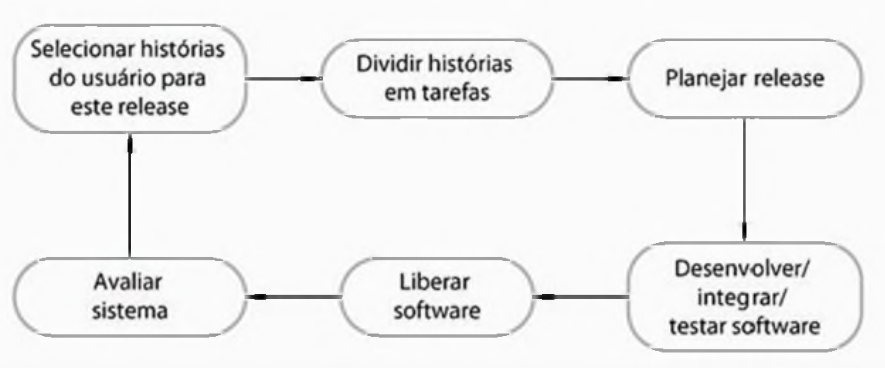
\includegraphics[scale=0.4]{src/tex/img/cicloReleaseXPSommerVille.png}\\
    \label{cicloRelease}
    \textbf{Fonte:} \citeonline{SOMMERVILLE:2011}
\end{figure}

As práticas necessárias para concluir um ciclo de \textit{release} do XP envolvem atividades desde o planejamento até especificações de como a equipe deve interagir. A primeira delas é o planejamento incremental, na qual se utiliza as histórias de usuário divididas em tarefas para realizar o planejamento de cada \textit{release}. É importante destacar que essas entregas devem ser pequenas, contínuas e contendo apenas o conjunto mínimo de funcionalidades úteis e isso reflete no princípio de que o projeto deve ser simples e apenas contemplar as atuais necessidades do cliente \cite{SOMMERVILLE:2011}.

Outra prática é o Desenvolvimento Orientado a Testes (TDD), ou seja, implementar primeiramente os testes automatizados e, após, a funcionalidade em si. No XP também é essencial que o código seja constantemente refatorado e melhorado. Esse método ágil também prevê a programação em pares (\textit{pair programming}), neste cenário os desenvolvedores trabalham em duplas, o que facilita a troca de conhecimento \cite{SOMMERVILLE:2011}.

No XP, o código deve ser de posse coletiva e, dessa forma, estabelece que esse pode ser modificado por qualquer membro da equipe sem a necessidade de permissão. Além disso, o desenvolvimento deve manter um ritmo sustentável, sem a exigência de muitas horas extras, que podem prejudicar a qualidade do produto. E, por fim, o XP considera o cliente como parte da equipe e ele deve estar disponível para diminuir possíveis barreiras de comunicação \cite{WAZLAWICK:2013}.

\subsection{\textit{Scrum}}
As bases do método ágil \textit{Scrum} foram definidas em 1986 a partir do artigo: "\textit{The New New Product Development Game} de \citeonline{Takeuchi:1986}. Esse artigo ilustrava o modelo de produção de automóveis da Honda que demonstrava algumas influências da filosofia \textit{Lean} \cite{WAZLAWICK:2013}.

Na área de desenvolvimento de \textit{software}, \textit{Scrum} é um \textit{framework} ágil formalizado por \citeonline{Sutherland:2013} através do "Um guia definitivo para o \textit{Scrum}: As regras do jogo". O nome do método tem origem em um termo de rúgbi e é um momento onde os jogadores se unem aos companheiros de time e trabalham em equipe para empurrar a bola em direção ao fundo do campo \cite{PRESSMAN:2011}. 

Segundo o Guia do \textit{Scrum} \cite{Sutherland:2013}, "o \textit{framework} \textit{Scrum} consiste nos times do Scrum associadas a papéis, eventos, artefatos e
regras." E, a partir desse \textit{framework}, as equipes podem resolver problemas complexos e adaptativos, ao mesmo tempo que garantem uma entrega de alto valor. 

Os papéis do time de \textit{Scrum} são: \textit{Scrum master} (mestre de \textit{Scrum}), \textit{product owner} (dono do produto) e \textit{development team} (equipe de desenvolvimento). O primeiro papel representa um membro da equipe com bastante conhecimento na aplicação do \textit{Scrum}. Apesar de representar um papel de lideranças, o \textit{Scrum} master não atua tal qual um gerente, ele age como um facilitador para aproximar a equipe das regras do \textit{Scrum} \cite{WAZLAWICK:2013}.

Já o \textit{product owner}, é o membro da equipe responsável pelo projeto e é quem define as funcionalidades a serem desenvolvidos a cada \textit{sprint}. Esse papel tem como objetivo identificar as necessidades do cliente e aplicá-las da maneira menos custosa possível. Por fim, o \textit{development team} são os membros que de fato desenvolvem o projeto, sem distinção entre papéis como desenvolvedores, analistas, \textit{designers} e testadores \cite{WAZLAWICK:2013}.

\citeonline{PRESSMAN:2011} destaca que o \textit{Scrum} utiliza um conjunto de padrões de processo que define um conjunto de ações de desenvolvimento. Esses padrões estão representados na Tabela abaixo e divididos em dois grupos: Eventos e Artefatos.

\begin{longtable}{|c|c|}
    \caption{Eventos e Artefatos do \textit{Scrum}}
    \label{tab:KeyComponents}
    \centering
              \centering
              \cr \rowcolor{lightgray}

            \textbf{Eventos} & \textbf{Artefatos} \\
            \hline 
            \textit{Sprint} & \textit{Product backlog}\\

            \textit{Sprint planning} & \textit{Sprint backlog}\\

            \textit{Daily scrum} & Incrementos\\

            \textit{Sprint review} & \\

            \textit{Sprint retrospective} & \\ \hline
            \addlinespace[0.2cm]
            \caption*{\textbf{Fonte:} Adaptado de \citeonline{PMIAGILE:2017}}
\end{longtable}

Os \textit{backlogs} são o registro de trabalhos pendentes. Consiste em uma lista priorizada com os requisitos a serem cumpridos \cite{PRESSMAN:2011}. O \textit{product backlog} costuma possuir histórias de usuário com uma descrição simples, um identificador e prioridade. Enquanto o \textit{sprint backlog} contém o plano daquela iteração corrente e já com os requisitos detalhados em formas de tarefas para as equipes de desenvolvimento realizarem. E, os incrementos são todo o trabalho realizado no período de uma \textit{sprint} \cite{WAZLAWICK:2013}.

As \textit{sprints} recebem esse nome por serem associadas à corridas de curta distância. Elas consistem em uma janela de tempo em que os trabalhos do \textit{sprint backlog} devem ser desenvolvidos. Elas ocorrem em forma de iterações, ao término o \textit{sprint backlog} é ajustado \cite{PRESSMAN:2011}.

Tratando agora das cerimônias do \textit{Scrum}, no começo de cada nova \textit{sprint} é feito o \textit{Sprint planning}, uma reunião na qual a equipe seleciona os elementos do \textit{product backlog} a serem desenvolvidos naquele ciclo. Essa reunião responde as perguntas: "O que pode ser entregue como resultado do incremento da próxima Sprint?" e "Como o trabalho necessário para entregar o incremento será realizado?" \cite{Sutherland:2013}.

A \textit{Daily scrum} é uma reunião diária que tem como o objetivo inspecionar o trabalho desenvolvido pela equipe desde a última \textit{Daily scrum} e também identificar obstáculos que estejam impedindo o progresso do time de desenvolvimento \cite{Sutherland:2013}. 

A \textit{Sprint review} e \textit{Sprint retrospective} devem ocorrer ao final de cada \textit{sprint}. A primeira, trata-se de uma avaliação do produto desenvolvido durante a \textit{sprint} e onde é feita a validação dos requisitos. Já a \textit{Sprint retrospective} trata da avaliação do processo de desenvolvimento e da equipe. A equipe, então, reflete sobre o passado e discute aquilo que deu certo e aquilo que precisa ser melhorado \cite{WAZLAWICK:2013}.

\subsection{Kanban}

\section{Guia para gestão ágil de riscos}


\chapter{Estado da arte}
\label{sec:EstadoArte}

O objetivo deste capítulo é apresentar o estado da arte do tema proposto por este trabalho. Para isso, foi realizada uma Revisão Sistemática da Literatura (RSL) nas bases de dados em conjunto com o trabalho de mestrado do aluno Fernando Vedoin Garcia. A RSL foi desenvolvida com base nas etapas propostas por \citeonline{Kitchenham:2004} no relatório "\textit{Procedures for performing systematic reviews}". 

O foco principal desta Revisão Sistemática da Literatura é identificar e analisar os atuais estudos empíricos sobre a aplicação de técnicas de gestão de riscos em contextos de desenvolvimento ágil. Levando em consideração quais técnicas foram aplicadas e os resultados obtidos a partir da aplicação.

\section{Revisão Sistemática da Literatura}

A realização da RSL utilizou as três etapas definidas por \citeonline{Kitchenham:2004}, identificadas abaixo: 

\begin{enumerate}
    \item Planejamento da revisão
        \begin{enumerate}
            \item Identificação da necessidade da revisão
            \item Desenvolvimento do protocolo de busca
        \end{enumerate}
    \item Condução da revisão
        \begin{enumerate}
            \item Identificação da pesquisa
            \item Seleção dos estudos primários
            \item Avaliação da qualidade dos estudos
            \item Extração de dados e monitoramento
            \item Sintetização dos dados
        \end{enumerate}
    \item Relatório da RSL
\end{enumerate}

\section{Definição do Protocolo de Revisão}

Com base nos objetivos da pesquisa identificada para este trabalho, foi definida a seguinte questão geral de pesquisa: "Quais são os resultados dos estudos empíricos de gestão de riscos em métodos ágeis?".

Após, foi utilizada a metodologia PICOC, sigla de População, Intervenção, Comparação, \textit{Outcome} (Resultado) e Contexto derivada da estratégia PICO utilizada na área médica \cite{SANTOS:2007}. Assim, foram definidos os seguintes elementos:

\begin{longtable}{|c|p{10cm}|}
    \caption{Descrição dos elementos PICOC}
    \label{tab:PICOCElements}
    \centering
              \centering
              \cr \rowcolor{lightgray}

            \textbf{Critérios} & \textbf{Descrição} 
            \\\hline 
            
            População & Organizações de \textit{software}.
            \\\hline
            
            Intervenção & Aplicação de técnicas de gerência de risco no contexto da organização.
            \\\hline

            Comparação & N/A
            \\\hline

            Resultado & Analisar se a qualidade do produto, prazo de entrega e características gerais do projeto foram impactadas.
            \\\hline

            Contexto & Utilização de métodos ágeis.
            \\\hline
            \addlinespace[0.2cm]
            \caption*{\textbf{Fonte:} Desenvolvido pela autora (2021).}
\end{longtable}

A partir da identificação dos elementos da Tabela \ref{tab:PICOCElements}, foram levantadas as seguintes questões de pesquisa: 

\begin{itemize} [label={}]
    \item \textbf{Q1.} Quais são os estudos que tratam de integração de práticas de gestão de riscos nos métodos ágeis?
    \item \textbf{Q2.} Qual contexto de uso de práticas de gestão de riscos nos métodos ágeis?
    \item \textbf{Q3.} Quais as características do ambiente de aplicação?
    \item \textbf{Q4.} Qual a motivação para a introdução de práticas explícitas de gestão de riscos nos métodos ágeis?
    \item \textbf{Q5.} Quais práticas de gestão de riscos são introduzidas nos métodos ágeis?
    \item \textbf{Q6.} Quais riscos são gerenciados?
    \item \textbf{Q7.} Quais os resultados da introdução de práticas explícitas de gestão de riscos nos métodos ágeis?
\end{itemize}

\section{Bases de dados}

\citeonline{Kitchenham:2004} destaca a importância do uso de bases de dados digitais para a área de Engenharia de \textit{Software}. Por isso, foram selecionadas três bibliotecas e bases de dados digitais relevantes para a área deste trabalho, são elas: ACM Digital Library, IEEExplore e Scopus. 

\section{Critérios de pesquisa}

Após a seleção das bases de dados, foram determinados critérios de busca para a seleção de artigos. Segundo \citeonline{Kitchenham:2004}, os estudos devem passar por uma série de estágios para serem escolhidos. O primeiro deles é aplicar os critérios de elegibilidade, após, filtra-se pelos títulos e resumos. Por fim, os trabalhos que não forem excluídos são analisados mais detalhadamente. Os critérios utilizados para realizar o primeiro filtro dos trabalhos foram:

\begin{itemize}
    \item Critérios de inclusão
        \begin{itemize}
            \item Estudos publicados em conferências, periódicos ou revistas científicas
            \item Estudos em Inglês ou Português.
            \item Artigos completos.
            \item Estudos publicados a partir de 2001.
        \end{itemize}
    \item Critérios de exclusão
        \begin{itemize}
            \item Estudos teóricos, não empíricos.
            \item Estudos duplicados.
            \item Estudos que não estejam acessíveis pela rede da Universidade Federal de Santa Catarina (UFSC).
            \item Estudos sem foco principal em desenvolvimento de \textit{software}.
        \end{itemize}
    \item Critérios de qualidade
        \begin{itemize}
            \item Estudos primários publicados que passaram por revisão por pares.
            \item Estudos do tipo empíricos.
            \item Estudos que deixem explícito quais foram as estratégias e técnicas adotadas na gestão de risco.
        \end{itemize}
\end{itemize}


\section{Termos de pesquisa}

Foram selecionados, então, os termos de buscas mais relevantes para o tema deste trabalho. A Tabela \ref{tab:ResearchTerms} apresenta os termos utilizados para refinar as buscas nas bases de dados e seus respectivos sinônimos. Entre eles estão \textit{software}, \textit{Risk management} e \textit{agile}. Os termos foram extraídos a partir de alguns elementos do PICOC. \\ \\

\begin{longtable}{|p{2.5cm}|p{4cm}|p{8cm}|}
    \caption{Termos de busca.}
    \label{tab:ResearchTerms}
    \centering
              \centering
              \cr \rowcolor{lightgray}
            \textbf{Critério} & \textbf{Termo} & \textbf{Sinônimos} 
            \\ \hline 
            
            \textbf{População} & \textit{Software} & N/A
            \\ \hline

            \textbf{Invervenção} & \textit{Risk Management} & \textit{Risk analysis, Risk administration, Management of risk}
            \\ \hline

            \textbf{Contexto} & \textit{Agile} & \textit{Scrum}, XP, \textit{Extreme Programming}, \textit{Lean}, Kanban, FDD, \textit{Feature Driven Development}, \textit{Crystal}, \textit{Iterative Development}
            \\ \hline 
            \addlinespace[0.2cm]
            \caption*{\textbf{Fonte:} Desenvolvido pela autora (2021).}
\end{longtable}

\section{\textit{Strings} de busca}

As \textit{strings} de busca sofreram adaptações para que retornassem resultados relacionados ao tema do presente trabalho. Na Tabela \ref{tab:StringsBusca} são apresentadas as \textit{strings} de busca utilizadas para cada base de dados.

\begin{longtable}{|c|p{11cm}|}
    \caption{\textit{Strings} de busca}
    \label{tab:StringsBusca}
    \centering
              \centering
              \cr \rowcolor{lightgray}

            \textbf{Base de dados} & \textbf{\textit{Strings} adaptadas} 
            \\ \hline 
            
            ACM Digital Library & (Abstract:(risk) AND Abstract:(agile OR scrum OR xp OR "extreme programming" OR lean OR kanban OR scrumban OR fdd OR "feature driven development" OR  Crystal OR "Iterative Development")) OR (Title:(risk) AND Title:(agile OR scrum OR xp OR "extreme programming" OR lean OR kanban OR scrumban OR fdd OR "feature driven development" OR  Crystal OR "Iterative Development"))
            \\ \hline
            
            IEEEXplore & All Metadata":risk AND ("All Metadata":agile OR "All Metadata":scrum OR "All Metadata":xp OR "All Metadata":"extreme programming" OR "All Metadata":lean OR "All Metadata":kanban OR "All Metadata":scrumban OR "All Metadata":fdd OR "All Metadata":“feature driven development” OR "All Metadata":Crystal OR "All Metadata":"Iterative Development")
            \\ \hline

            Scopus & (TITLE-ABS-KEY (risk) AND (TITLE-ABS-KEY(agile) OR TITLE-ABS-KEY (scrum) OR TITLE-ABS-KEY (xp) OR TITLE-ABS-KEY (extreme AND programming) OR TITLE-ABS-KEY (lean) OR TITLE-ABS-KEY (kanban) OR TITLE-ABS-KEY (scrumban) OR TITLE-ABS-KEY (fdd) OR TITLE-ABS-KEY (feature AND driven AND development) OR TITLE-ABS-KEY (crystal) OR TITLE-ABS-KEY (iterative AND development)) AND (LIMIT-TO (SUBJAREA,"COMP")))
            \\ \hline

            \addlinespace[0.2cm]
            \caption*{\textbf{Fonte:} Desenvolvido pela autora (2021).}
\end{longtable}

As bases de dados retornaram no total 3339 estudos após a aplicação das \textit{strings}. E, os estudos foram distribuídos conforme a Figura \ref{EstudosRetornados}.

\begin{figure}[h]
    \centering
    \caption{Estudos retornados em cada base de dados}
    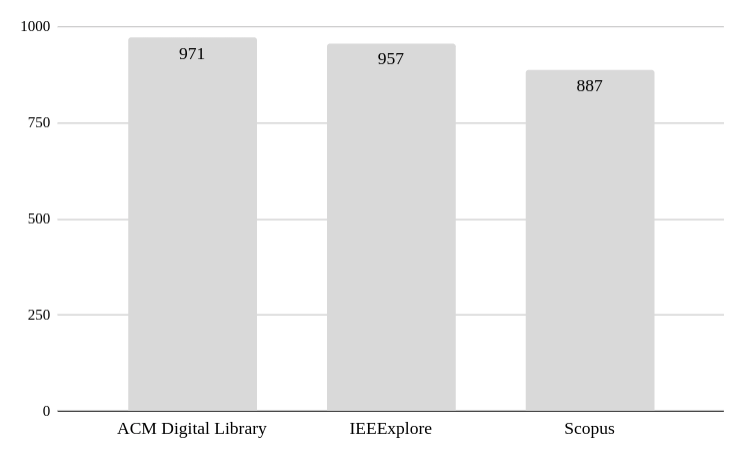
\includegraphics[scale=0.55]{src/tex/img/graficoBuscas.png} \\
    \label{EstudosRetornados}
    \textbf{Fonte:} Desenvolvido pela autora (2021).
    \centering
\end{figure}

\section{Seleção dos artigos}

Mesmo com as \textit{strings} de busca limitando o conteúdo dos estudos retornados, ainda assim as buscas resultaram em um volume grande de estudos. Por isso, foi realizada uma filtragem através da leitura dos títulos.

A partir dos artigos restantes, fez-se uma segunda filtragem que teve como critério a leitura dos resumos e a estrutura geral dos artigos. Desta forma, foi possível aplicar os critérios de inclusão, exclusão e qualidade para cada um deles. 

Enfim, após a segunda filtragem, foi realizada a leitura integral do texto de cada trabalho. Com base nesta leitura, foi possível identificar aqueles mais relevantes com base nas perguntas de pesquisa. Esses, então, foram selecionados para a extração e análise dos dados.

\section{Extração de dados}

Para realizar a coleta de dados, foram selecionados dados relevantes a serem levantados nos artigos com base nas perguntas de pesquisa. A partir de tais dados, foram criadas questões de análise. As questões foram definidas segundo a Tabela \ref{tab:QAnalise}.

\begin{longtable}{|p{8cm}|p{5cm}|}
    \caption{Questões de análise.}
    \label{tab:QAnalise}
    \centering
            \centering
            \cr \rowcolor{lightgray}
            \textbf{Questão de pesquisa} & \textbf{Questões de análise} 
            \\ \hline 
            
            \multirow{1}{12em}{\textbf{Q2.} Qual contexto de uso de práticas de gestão de riscos nos métodos ágeis?}
            & \textbf{Q2.1} Contexto de uso \\
            & \textbf{Q2.2} Método Ágil \\
            & \textbf{Q2.3} Tipo do estudo
            \\ \hline
            
            \multirow{1}{12em}{\textbf{Q3.} Quais as características do ambiente de aplicação?}
            & \textbf{Q3.1} Tamanho da equipe \\
            & \textbf{Q3.2} Domínio da aplicação \\
            & \textbf{Q3.3} Tipo do produto 
            \\ \hline
            
            \multirow{1}{12em}{\textbf{Q5.} Quais práticas de gestão de riscos são introduzidas nos métodos ágeis?}
            & \textbf{Q5.1} Lista de práticas \\ & \\ & \\ &
            \\ \hline
            
            \multirow{1}{12em}{\textbf{Q6.} Quais riscos são gerenciados?}
            & \textbf{Q6.1} Lista de riscos \\ & 
            \\ \hline
            
            \multirow{1}{12em}{\textbf{Q7.} Quais os resultados da introdução de práticas explícitas de gestão de riscos nos métodos ágeis?}
            & \textbf{Q6.1} Lista de resultados \\ & \\ & \\ &
            \\ \hline
\end{longtable}

\section{Análise dos resultados}

Nesta seção foi realizada a síntese e classificação dos estudos selecionados, estes estão numerados e referenciados no Apêndice \ref{sec:ApendiceA}.

\begin{longtable}{|p{4cm}|p{4cm}|p{8cm}|}
    \caption{Classificação dos estudos.}
    \label{tab:ClassificacaoEstudos}
    \centering
             \centering
             \cr \rowcolor{lightgray}
            \multicolumn{2}{|c|}{\textbf{Classificação}} & \textbf{Estudos} 
            \\ \hline 
            
            \multirow{1}{10em}{Contexto de uso}
            & Indústria & [1], [2], [3], [4], [5], [8], [9], [11], [13], [14], [15], [16], [17], [18], [19] \\ 
            & Academia & [6], [7], [10], [12]
            \\ \hline
            
            \multirow{1}{10em}{Métodos ágeis utilizados no estudo}
            & \textit{Scrum} & [3], [5], [6], [7], [10], [11], [13], [18] \\ 
            & Kanban & [9], [18] \\ 
            & XP & [1], [13], [15], [18] \\
            & DSDM & [13] \\
            & Lean & [14] \\
            & Não informado & [2], [4], [8], [12], [16], [17], [19]
            \\ \hline
            
            \multirow{1}{10em}{Tipo do estudo}
            & Experimento & [1], [10], [11], [12] \\ 
            & Estudo de caso & [2], [3], [4], [5], [6], [8], [13], [14], [15], [16], [17], [18], [19] \\ 
            & Prova de conceito & [9] 
            \\ \hline
            
            \multirow{1}{10em}{Tamanho da equipe}
            & <10 & [3], [5], [6], [7], [11], [12], [15], [16]\\ 
            & >10 & [4], [5], [11] \\ 
            & Não informado & [1], [2], [8], [10], [13], [14], [17], [18], [19]
            \\ \hline
            
            \multirow{1}{10em}{Domínio da aplicação}
            & Militar & [2]\\ 
            & Financeiro & [3] \\ 
            & \textit{E-commerce} & [4], [7], [9] \\
            & Múltiplos domínios & [8], [13], [14] \\
            & Gestão & [15], [16], [18] \\
            & Saúde & [17], [18] \\
            & Telecomunicação & [19] \\
            & Não informado & [1], [5], [6], [10], [11], [12]
            \\ \hline
            
            \multirow{1}{10em}{Tamanho do produto}
            & Grande & [2], [3], [4], [8], [9], [13], [14], [17], [18], [19] \\ 
            & Pequeno & [6], [7] \\ 
            & Não informado & [1], [5], [10], [11], [12], [15]
            \\ \hline
            
            \multirow{1}{10em}{Tipo do produto}
            & \textit{Mobile} & [16]\\ 
            & Web & [2], [7], [16], [19] \\ 
            & Misto & [1], [18] \\
            & \textit{Hardware e software} & [17] \\
            & Não informado & [3], [4], [5], [6], [8], [9], [10], [11], [12], [13], [14], [15]
            \\ \hline
        
            \addlinespace[0.2cm]
            \caption*{\textbf{Fonte:} Desenvolvido pela autora (2021).}
\end{longtable}

\subsection{Contexto das organizações}

\subsection{Métodos ágeis utilizados}

\subsection{Práticas de gestão de riscos adotadas}

\subsection{Riscos gerenciados}

\subsection{Resultados obtidos com os estudos}

\section{Ameaças à validade}



\chapter{Processo Atual da Organização}
\label{sec:Processo}


\chapter{Proposta do Trabalho}
\label{sec:Proposta}


\chapter{Experimentos e Discussão}
\label{sec:Experimentos}


\chapter{Conclusões e Trabalhos Futuros}
\label{sec:Conclusoes}


  \postextual


  % ----------------------------------------------------------
  % Referências bibliográficas
  % ----------------------------------------------------------
  \bibliography{references}
  
  % ----------------------------------------------------------
  % Glossário
  % ----------------------------------------------------------
  %
  % Consulte o manual da classe abntex2 para orientações sobre o glossário.
  %
  %\glossary

  % ----------------------------------------------------------
  % Apêndices
  % ----------------------------------------------------------

  % ---
  % Inicia os apêndices
  % ---
  \begin{apendicesenv}
    
  % Imprime uma página indicando o início dos apêndices
  \partapendices
  % ----------------------------------------------------------
 \chapter{Estudos Selecionados na Revisão Sistemática da Literatura}
 \label{sec:ApendiceA}
 
 O quadro abaixo apresenta os estudos selecionados durante a Revisão Sistemática da Literatura.

\begin{longtable}{|p{1cm}|p{4cm}|p{9.5cm}|}
    \centering
            \rowcolor{lightgray}
            \textbf{ID} & \textbf{Título} & \textbf{Referência} 
            \\ \hline 
            
            \flushleft{\textbf{[1]}} & \flushleft{\textit{Identifying Risks in XP Projects through Process Modelling}} & \flushleft{KIRK, D.; TEMPERO, E.. Identifying risks in XP projects through process modelling. \textbf{Australian Software Engineering Conference (Aswec'06)}, [S.L.], p. 10-420, 2006. IEEE. http://dx.doi.org/10.1109/aswec.2006.31.}
            \\ \hline

            \flushleft{\textbf{[2]}} & \flushleft{\textit{Reference framework and model for integration of risk management in agile systems engineering lifecycle of the defense acquisition management framework}} & \flushleft{CROWE, Portia; MOSTASHARI, Ali; MANSOURI, Mo; CLOUTIER, Robert. 9.2.1 Reference Framework and Model for Integration of Risk Management in Agile Systems Engineering Lifecycle of the Defense Acquisition Management Framework. \textbf{Incose International Symposium}, [S.L.], v. 19, n. 1, p. 1391-1405, jul. 2009. Wiley. http://dx.doi.org/10.1002/j.2334-5837.2009.tb01022.x.}
            \\ \hline

            \flushleft{\textbf{[3]}} & \flushleft{\textit{A risk management framework for distributed scrum using prince2 methodology}} & \flushleft{ESTEKI, Mohammad; GANDOMANI, Taghi Javdani; FARSANI, Hadi Khosravi. A risk management framework for distributed scrum using PRINCE2 methodology. \textbf{Bulletin Of Electrical Engineering And Informatics}, [S.L.], v. 9, n. 3, p. 1299-1310, 1 jun. 2020. Institute of Advanced Engineering and Science. http://dx.doi.org/10.11591/eei.v9i3.1905.}
            \\ \hline \hline
            
            \flushleft{\textbf{[4]}} & \flushleft{\textit{Improving Risk Management in a Scaled Agile Environment}} & \flushleft{SCHÖN, Eva-Maria; RADTKE, Dirk; JORDAN, Christian. Improving Risk Management in a Scaled Agile Environment. \textbf{Lecture Notes In Business Information Processing}, [S.L.], p. 132-141, 2020. Springer International Publishing. http://dx.doi.org/10.1007/978-3-030-49392-99}
            \\ \hline        
 
            \flushleft{\textbf{[5]}} & \flushleft{\textit{Risk assessment forum: A proposal for agile software development teams ruled by Scrum}} & \flushleft{CARVALLO, Juliette Michelle Parada; OKTABA, Hanna; HERNANDEZ, Elsa Ramirez. Risk Assessment Forum. \textbf{2018 6Th International Conference In Software Engineering Research And Innovation (Conisoft)}, [S.L.], p. 132-141, out. 2018. IEEE. http://dx.doi.org/10.1109/conisoft.2018.8645949.}
            \\ \hline
            
            \flushleft{\textbf{[6]}} & \flushleft{\textit{Agile risk management using software agents}} & \flushleft{ODZALY, Edzreena Edza; GREER, Des; STEWART, Darryl. Agile risk management using software agents. \textbf{Journal Of Ambient Intelligence And Humanized Computing}, [S.L.], v. 9, n. 3, p. 823-841, 2 maio 2017. Springer Science and Business Media LLC. http://dx.doi.org/10.1007/s12652-017-0488-2.}
            \\ \hline                

            \flushleft{\textbf{[7]}} & \flushleft{\textit{A risk poker based testing model for scrum}} & \flushleft{GHAZALI, Siti Noor Hasanah; SALIM, Siti Salwah; INAYAT, Irum; HAMID, Siti Hafizah Ab. A Risk Poker Based Testing Model for Scrum. \textbf{Computer Systems Science And Engineering}, [S.L.], v. 33, n. 3, p. 169-185, 2018. Computers, Materials and Continua (Tech Science Press). http://dx.doi.org/10.32604/csse.2018.33.169.} 
            \\ \hline \hline
            
            \flushleft{\textbf{[8]}} & \flushleft{\textit{Characterization and prediction of issue-related risks in software projects}} & \flushleft{CHOETKIERTIKUL, Morakot; DAM, Hoa Khanh; TRAN, Truyen; GHOSE, Aditya. Characterization and Prediction of Issue-Related Risks in Software Projects. \textbf{2015 Ieee/Acm 12Th Working Conference On Mining Software Repositories}, [S.L.], maio 2015. IEEE. http://dx.doi.org/10.1109/msr.2015.33.}
            \\ \hline    
            
            \flushleft{\textbf{[9]}} & \flushleft{\textit{Agile approach with Kanban in information security risk management}} & \flushleft{DORCA, Vasile; MUNTEANU, Radu; POPESCU, Sorin; CHIOREANU, Adrian; PELESKEI, Claudius. Agile approach with Kanban in information security risk management. \textbf{2016 Ieee International Conference On Automation, Quality And Testing, Robotics (Aqtr)}, [S.L.], p. 1-6, maio 2016. IEEE. http://dx.doi.org/10.1109/aqtr.2016.7501278.}
            \\ \hline                
            
            \flushleft{\textbf{[10]}} & \flushleft{\textit{Integrating Risk Management in Scrum Framework}} & \flushleft{HAMMAD, Muhammad; INAYAT, Irum. Integrating Risk Management in Scrum Framework.\textbf{ 2018 International Conference On Frontiers Of Information Technology (Fit)}, [S.L.], p. 158-163, dez. 2018. IEEE. http://dx.doi.org/10.1109/fit.2018.00035.}
            \\ \hline                
            
            \flushleft{\textbf{[11]}} & \flushleft{\textit{Risk Assessment Forum}} & \flushleft{CARVALLO, Juliette Michelle Parada; OKTABA, Hanna; HERNANDEZ, Elsa Ramirez. Risk Assessment Forum. \textbf{2018 6Th International Conference In Software Engineering Research And Innovation (Conisoft)}, [S.L.], out. 2018. IEEE. http://dx.doi.org/10.1109/conisoft.2018.8645949.}
            \\ \hline \hline

            \flushleft{\textbf{[12]}} & \flushleft{\textit{A Risk Management Tool for Agile Software Development}} & \flushleft{TAVARES, Breno Gontijo; KEIL, Mark; SILVA, Carlos Eduardo Sanches da; SOUZA, Adler Diniz de. A Risk Management Tool for Agile Software Development. \textbf{Journal Of Computer Information Systems}, [S.L.], p. 1-10, 7 dez. 2020. Informa UK Limited. http://dx.doi.org/10.1080/08874417.2020.1839813.}
            \\ \hline

            \flushleft{\textbf{[13]}} & \flushleft{\textit{Prioritizing and optimizing risk factors in agile software development}} & \flushleft{ AGRAWAL, Ruchi; SINGH, Deepali; SHARMA, Ashish. Prioritizing and optimizing risk factors in agile software development. \textbf{2016 Ninth International Conference On Contemporary Computing (Ic3)}, [S.L.], p. 1-7, ago. 2016. IEEE. http://dx.doi.org/10.1109/ic3.2016.7880232.}
            \\ \hline 
            
            \flushleft{\textbf{[14]}} & \flushleft{\textit{Identifying risky areas of software code in Agile/Lean software development: An industrial experience report}} & \flushleft{ANTINYAN, Vard; STARON, Miroslaw; MEDING, Wilhelm; OSTERSTROM, Per; WIKSTROM, Erik; WRANKER, Johan; HENRIKSSON, Anders; HANSSON, Jorgen. Identifying risky areas of software code in Agile/Lean software development: an industrial experience report. \textbf{2014 Software Evolution Week - Ieee Conference On Software Maintenance, Reengineering, And Reverse Engineering (Csmr-Wcre)}, [S.L.], p. 154-163, fev. 2014. IEEE. http://dx.doi.org/10.1109/csmr-wcre.2014.6747165.}
            \\ \hline \hline       
 
            \flushleft{\textbf{[15]}} & \flushleft{\textit{Value-Risk Trade-off Analysis for Iteration Planning in Extreme Programming}} & \flushleft{DONG, Xin; YANG, Qiu-Song; WANG, Qing; ZHAI, Jian; RUHE, Gunther. Value-Risk Trade-off Analysis for Iteration Planning in Extreme Programming. \textbf{2011 18Th Asia-Pacific Software Engineering Conference}, [S.L.], p. 397-404, dez. 2011. IEEE. http://dx.doi.org/10.1109/apsec.2011.11.}
            \\ \hline    
            
            \flushleft{\textbf{[16]}} & \flushleft{\textit{A case study for the implementation of an agile risk management process in multiple projects environments}} & \flushleft{RIBEIRO, Lucio; GUSMAO, Cristine; FEIJO, Wilmar; BEZERRA, Vicente. A case study for the implementation of an agile risk management process in multiple projects environments. \textbf{Picmet '09 - 2009 Portland International Conference On Management Of Engineering \& Technology}, [S.L.], p. 1396-1404, ago. 2009. IEEE. http://dx.doi.org/10.1109/picmet.2009.5262002.}
            \\ \hline                

            \flushleft{\textbf{[17]}} & \flushleft{\textit{A SYSML-Based Approach for Requirements Risk Management and Change Control}} & \flushleft{HAYAT, Faisal; ANWAR, Muhammad Waseem; AZAM, Farooque; KIRAN, Ayesha. A SYSML-Based Approach for Requirements Risk Management and Change Control. Proceedings Of The 2019 11Th International Conference On Information Management And Engineering, [S.L.], p. 20-24, 19 set. 2019. ACM. http://dx.doi.org/10.1145/3373744.3373751.}
            \\ \hline \hline   
            
            \flushleft{\textbf{[18]}} & \flushleft{\textit{Risk Management for Agile Projects in Offshore Vietnam}} & \flushleft{CUONG, Le Gia; HUNG, Phan Duy; BACH, Nguyen Luu; TUNG, Ta Duc. Risk Management for Agile Projects in Offshore Vietnam. \textbf{Proceedings Of The Tenth International Symposium On Information And Communication Technology - Soict 2019}, [S.L.], p. 377-384, 2019. ACM Press. http://dx.doi.org/10.1145/3368926.3369718.}
            \\ \hline    
            
            \flushleft{\textbf{[19]}} & \flushleft{\textit{An industrial case study of implementing software risk management}} & \flushleft{FREIMUT, Bernd; HARTKOPF, Susanne; KAISER, Peter; KONTIO, Jyrki; KOBITZSCH, Werner. An industrial case study of implementing software risk management. \textbf{Acm Sigsoft Software Engineering Notes}, [S.L.], v. 26, n. 5, p. 277-287, set. 2001. Association for Computing Machinery (ACM). http://dx.doi.org/10.1145/503271.503247.}
            \\ \hline                
            
            \addlinespace[0.2cm]
            \caption*{\textbf{Fonte:} Desenvolvido pela autora (2021).}
\end{longtable}


  \end{apendicesenv}
  % ---


  % ----------------------------------------------------------
  % Anexos
  % ----------------------------------------------------------

  % ---
  % Inicia os anexos
  % ---
  % \begin{anexosenv}

  % Imprime uma página indicando o início dos anexos
  % \partanexos

  % ---
  % \chapter{Morbi ultrices rutrum lorem.}
  % ---
  % \lipsum[30]

  % ---
  % \chapter{Cras non urna sed feugiat cum sociis natoque penatibus et magnis dis
  % parturient montes nascetur ridiculus mus}
  % ---

  % \lipsum[31]

  % ---
  % \chapter{Fusce facilisis lacinia dui}
  % ---

  % \lipsum[32]

  % \end{anexosenv}

  %---------------------------------------------------------------------
  % INDICE REMISSIVO
  %---------------------------------------------------------------------

  \printindex

  \end{document}
